\documentclass[12pt]{article}
\usepackage{amsthm,amssymb,amsfonts,amsmath,amstext,systeme,adjustbox}
\usepackage{graphicx,float,wrapfig}
\usepackage{tabularx,enumitem}
\marginparwidth 0pt
\oddsidemargin -1.2 truecm
\evensidemargin  0pt 
\marginparsep 0pt
\topmargin -2.2truecm
\linespread{1}
\textheight 25.8 truecm
\textwidth 18.5 truecm
\newenvironment{remark}{\noindent{\bf Remark }}{\vspace{0mm}}
\newenvironment{remarks}{\noindent{\bf Remarks }}{\vspace{0mm}}
\newenvironment{question}{\noindent{\bf Question }}{\vspace{0mm}}
\newenvironment{questions}{\noindent{\bf Questions }}{\vspace{0mm}}
\newenvironment{note}{\noindent{\bf Note }}{\vspace{0mm}}
\newenvironment{summary}{\noindent{\bf Summary }}{\vspace{0mm}}
\newenvironment{back}{\noindent{\bf Background}}{\vspace{0mm}}
\newenvironment{conclude}{\noindent{\bf Conclusion}}{\vspace{0mm}}
\newenvironment{concludes}{\noindent{\bf Conclusions}}{\vspace{0mm}}
\newenvironment{dill}{\noindent{\bf Description of Dill's model}}{\vspace{0mm}}
\newenvironment{maths}{\noindent{\bf Mathematics needed}}{\vspace{0mm}}
\newenvironment{inst}{\noindent{\bf Instructions}}{\vspace{0mm}}
\newenvironment{notes}{\noindent{\bf Notes }}{\vspace{0mm}}
\newenvironment{theorem}{\noindent{\bf Theorem }}{\vspace{0mm}}
\newenvironment{example}{\noindent{\bf Example }}{\vspace{0mm}}
\newenvironment{examples}{\noindent{\bf Examples }}{\vspace{0mm}}
\newenvironment{topics}{\noindent{\bf Topics}}{\vspace{0mm}}
\newenvironment{outcomes}{\noindent{\bf Expected Learning Outcomes}}{\vspace{0mm}}
\newenvironment{lemma}{\noindent{\bf Lemma }}{\vspace{0mm}}
\newenvironment{solution}{\noindent{\it Solution}}{\vspace{2mm}}
\newcommand{\ds}{\displaystyle}
\newcommand{\un}{\underline}
\newcommand{\bs}{\boldsymbol}

\begin{document}

\baselineskip 18 pt
\begin{center}
	{\large \bf HKDSE MATH Core Sample Paper II}\\
	\vspace{2 mm}
\end{center}
\vspace{0.05cm}

\begin{enumerate}
	\item \textbf{HKDSE MATH Core Sample Paper II Q1}\\
	$(3a)^2 \cdot a^3 = $
	\begin{enumerate}
		\item[A.] $3a^5$.
		\item[B.] $6a^6$.
		\item[C.] $9a^5$.
		\item[D.] $9a^6$.
	\end{enumerate}

	\item \textbf{HKDSE MATH Core Sample Paper II Q2}\\
	If $5 - 3m = 2n$, then $m =$
	\begin{enumerate}
		\item[A.] $n$.
		\item[B.] $\dfrac{2n - 5}{3}$.
		\item[C.] $\dfrac{-2n + 5}{3}$.
		\item[D.] $\dfrac{-2n + 15}{3}$.
	\end{enumerate}

	\item \textbf{HKDSE MATH Core Sample Paper II Q3}\\
	$a^2 - b^2 + 2b - 1 =$
	\begin{enumerate}
		\item[A.] $(a - b - 1)(a + b - 1)$
		\item[B.] $(a - b - 1)(a + b + 1)$
		\item[C.] $(a - b + 1)(a + b - 1)$
		\item[D.] $(a - b + 1)(a - b - 1)$
	\end{enumerate}

	\item \textbf{HKDSE MATH Core Sample Paper II Q4}\\
	Let $p$ and $q$ be constants. If $x^2 + p(x + 5) + q \equiv (x - 2)(x + 5)$, then $q = $
	\begin{enumerate}
		\item[A.] $-25$.
		\item[B.] $-10$.
		\item[C.] $3$.
		\item[D.] $5$.
	\end{enumerate}

	\item \textbf{HKDSE MATH Core Sample Paper II Q5}\\
	Let $f(x) = x^3 + 2x^2 - 7x + 3$. When $f(x)$ is divided by $x + 2$, the remainder is 
	\begin{enumerate}
		\item[A.] 3.
		\item[B.] 5.
		\item[C.] 17.
		\item[D.] 33.
	\end{enumerate}

	\item \textbf{HKDSE MATH Core Sample Paper II Q6}\\
	Let $a$ be a constant. Solve tne equation $(x - a)(x - a - 1) = (x - a)$.
	\begin{enumerate}
		\item[A.] $x = a + 1$
		\item[B.] $x = a + 2$
		\item[C.] $x = a$ or $x = a + 1$
		\item[D.] $x = a$ or $x = a + 2$
	\end{enumerate}

	\item \textbf{HKDSE MATH Core Sample Paper II Q7}\\
	Find the range of values of $k$ such that the quadratic equation $x^2 - 6x = 2 - k$ has no real roots.
	\begin{enumerate}
		\item[A.] $k < -7$
		\item[B.] $k > -7$
		\item[C.] $k < 11$
		\item[D.] $k > 11$
	\end{enumerate}

	\item \textbf{HKDSE MATH Core Sample Paper II Q8}\\
	In the figure, the quadratic graph of $y = f(x)$ intersects the straight line $L$ at $A(1 , k)$ and $B(7 , k)$. Which of the following are true?
	\begin{enumerate}
		\item[I.] The solution of the inequality $f(x) > k$ is $x < 1$ or $x > 7$.
		\item[II.] The roots of the equation $f(x) = k$ are 1 and 7.
		\item[III.] The equation of the axis of symmetry of the quadratic graph of $y = f(x)$ is $x = 3$.
		\item[]
		% \begin{figure}[h]
		% 	\centering
		% 	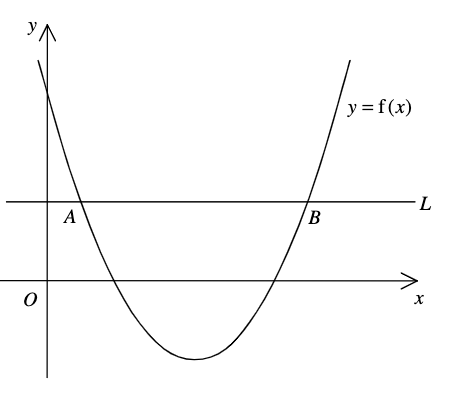
\includegraphics[width = .4\textwidth]{SPFigure2.8.png}
		% \end{figure}

		% \begin{enumerate}
		% 	\item[A.] I and II only
		% 	\item[B.] I and III only
		% 	\item[C.] II and III only
		% 	\item[D.] I, II and III
		% \end{enumerate}


		\begin{minipage}[p]{.3\textwidth}
			\begin{enumerate}[label=(\Alph*), itemsep=0pt]
				\item[A.] I and II only
				\item[B.] I and III only
				\item[C.] II and III only
				\item[D.] I, II and III
			\end{enumerate}
		\end{minipage}
		\begin{minipage}[b]{.5\textwidth}
			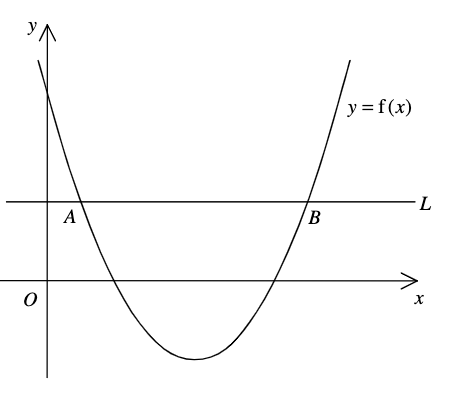
\includegraphics[scale=0.7]{SPFigure2.8.png}
		\end{minipage}
	\end{enumerate}
		
	\item \textbf{HKDSE MATH Core Sample Paper II Q9}\\
	The solution of $5 - 2x < 3$ and $4x + 8 > 0$ is 
	\begin{enumerate}
		\item[A.] $x > -2$.
		\item[B.] $x > -1$.
		\item[C.] $x > 1$.
		\item[D.] $-2 < x < 1$.
	\end{enumerate}

	\item \textbf{HKDSE MATH Core Sample Paper II Q10}\\
	Mary sold two bags for \$240 each. She gained 20\% on one and lost 20\% on the other. After the two transactions, Mary
	\begin{enumerate}
		\item[A.] lost \$20.
		\item[B.] gained \$10.
		\item[C.] gained \$60.
		\item[D.] had no gain and no loss.
	\end{enumerate}

	\item \textbf{HKDSE MATH Core Sample Paper II Q11}\\
	Let $a_n$ be the $n$th term of a sequence. If $a_1 = 4$, $a_2 = 5$ and $a_{n + 2} = a_n + a_{n + 1}$ for any positive integer $n$, then $a_{10} = $
	\begin{enumerate}
		\item[A.] 13.
		\item[B.] 157.
		\item[C.] 254.
		\item[D.] 411.
	\end{enumerate}

	\item \textbf{HKDSE MATH Core Sample Paper II Q12}\\
	If the length and the width of a rectangle are increased by 20\% and $x\%$ respectively so that its area is increased by 50\%, then $x = $
	\begin{enumerate}
		\item[A.] 20.
		\item[B.] 25.
		\item[C.] 30.
		\item[D.] 35.
	\end{enumerate}

	\item \textbf{HKDSE MATH Core Sample Paper II Q13}\\
	If $x$, $y$ and $z$ are non-zero numbers such that $2x = 3y$ and $x = 2z$, then $(x + z) : (x + y) = $
	\begin{enumerate}
		\item[A.] 3 : 5.
		\item[B.] 6 : 7.
		\item[C.] 9 : 7.
		\item[D.] 9 : 10.
	\end{enumerate}

	\item \textbf{HKDSE MATH Core Sample Paper II Q14}\\
	It is given that $z$ varies directly as $x$ and inversely as $y$. When $x = 3$ and $y = 4$ , $z = 18$ . When $x = 2$ and $z = 8$, $y = $
	\begin{enumerate}
		\item[A.] 1.
		\item[B.] 3.
		\item[C.] 6.
		\item[D.] 9.
	\end{enumerate}

	\item \textbf{HKDSE MATH Core Sample Paper II Q15}\\
	The lengths of the three sides of a triangle are measured as 15 cm, 24 cm and 25 cm respectively. If the three measurements are correct to the nearest cm , find the percentage error in calculating the perimeter of the triangle correct to the nearest 0.1\%.
	\begin{enumerate}
		\item[A.] 0.8\%
		\item[B.] 2.3\%
		\item[C.] 4.7\%
		\item[D.] 6.3\%
	\end{enumerate}

	\item \textbf{HKDSE MATH Core Sample Paper II Q16}\\
	In the figure, $O$ is the centre of the circle. $C$ and $D$ are points lying on the circle. $OBC$ and $BAD$ are straight lines. If $)C = 20$ cm and $OA = AB = 10$ cm, find the area of the shaded region $BCD$ correct to the nearest cm$^2$.
	\begin{enumerate}
		\item[A.] 214 cm$^2$
		\item[B.] 230 cm$^2$
		\item[C.] 246 cm$^2$
		\item[D.] 270 cm$^2$
	\end{enumerate}

	\item \textbf{HKDSE MATH Core Sample Paper II Q17}\\
	
	\begin{enumerate}
		\item[A.]
		\item[B.]
		\item[C.]
		\item[D.]
	\end{enumerate}

	\item \textbf{HKDSE MATH Core Sample Paper II Q18}\\
	
	\begin{enumerate}
		\item[A.]
		\item[B.]
		\item[C.]
		\item[D.]
	\end{enumerate}

	\item \textbf{HKDSE MATH Core Sample Paper II Q19}\\
	
	\begin{enumerate}
		\item[A.]
		\item[B.]
		\item[C.]
		\item[D.]
	\end{enumerate}

	\item \textbf{HKDSE MATH Core Sample Paper II Q20}\\
	
	\begin{enumerate}
		\item[A.]
		\item[B.]
		\item[C.]
		\item[D.]
	\end{enumerate}

	\item \textbf{HKDSE MATH Core Sample Paper II Q21}\\
	
	\begin{enumerate}
		\item[A.]
		\item[B.]
		\item[C.]
		\item[D.]
	\end{enumerate}

	\item \textbf{HKDSE MATH Core Sample Paper II Q22}\\
	
	\begin{enumerate}
		\item[A.]
		\item[B.]
		\item[C.]
		\item[D.]
	\end{enumerate}

	\item \textbf{HKDSE MATH Core Sample Paper II Q23}\\
	
	\begin{enumerate}
		\item[A.]
		\item[B.]
		\item[C.]
		\item[D.]
	\end{enumerate}

	\item \textbf{HKDSE MATH Core Sample Paper II Q24}\\
	
	\begin{enumerate}
		\item[A.]
		\item[B.]
		\item[C.]
		\item[D.]
	\end{enumerate}

	\item \textbf{HKDSE MATH Core Sample Paper II Q25}\\
	
	\begin{enumerate}
		\item[A.]
		\item[B.]
		\item[C.]
		\item[D.]
	\end{enumerate}
	\item \textbf{HKDSE MATH Core Sample Paper II Q26}\\
	\begin{enumerate}
		\item[A.]
		\item[B.]
		\item[C.]
		\item[D.]
	\end{enumerate}
	\item \textbf{HKDSE MATH Core Sample Paper II Q27}\\
	\begin{enumerate}
		\item[A.]
		\item[B.]
		\item[C.]
		\item[D.]
	\end{enumerate}
	\item \textbf{HKDSE MATH Core Sample Paper II Q28}\\
	\begin{enumerate}
		\item[A.]
		\item[B.]
		\item[C.]
		\item[D.]
	\end{enumerate}
	\item \textbf{HKDSE MATH Core Sample Paper II Q29}\\
	\begin{enumerate}
		\item[A.]
		\item[B.]
		\item[C.]
		\item[D.]
	\end{enumerate}
	\item \textbf{HKDSE MATH Core Sample Paper II Q30}\\
	\begin{enumerate}
		\item[A.]
		\item[B.]
		\item[C.]
		\item[D.]
	\end{enumerate}
	\item \textbf{HKDSE MATH Core Sample Paper II Q31}\\
	\begin{enumerate}
		\item[A.]
		\item[B.]
		\item[C.]
		\item[D.]
	\end{enumerate}
	\item \textbf{HKDSE MATH Core Sample Paper II Q32}\\
	\begin{enumerate}
		\item[A.]
		\item[B.]
		\item[C.]
		\item[D.]
	\end{enumerate}
	\item \textbf{HKDSE MATH Core Sample Paper II Q33}\\
	\begin{enumerate}
		\item[A.]
		\item[B.]
		\item[C.]
		\item[D.]
	\end{enumerate}
	\item \textbf{HKDSE MATH Core Sample Paper II Q34}\\
	\begin{enumerate}
		\item[A.]
		\item[B.]
		\item[C.]
		\item[D.]
	\end{enumerate}
	\item \textbf{HKDSE MATH Core Sample Paper II Q35}\\
	\begin{enumerate}
		\item[A.]
		\item[B.]
		\item[C.]
		\item[D.]
	\end{enumerate}
	\item \textbf{HKDSE MATH Core Sample Paper II Q36}\\
	\begin{enumerate}
		\item[A.]
		\item[B.]
		\item[C.]
		\item[D.]
	\end{enumerate}
	\item \textbf{HKDSE MATH Core Sample Paper II Q37}\\
	\begin{enumerate}
		\item[A.]
		\item[B.]
		\item[C.]
		\item[D.]
	\end{enumerate}
	\item \textbf{HKDSE MATH Core Sample Paper II Q38}\\
	\begin{enumerate}
		\item[A.]
		\item[B.]
		\item[C.]
		\item[D.]
	\end{enumerate}
	\item \textbf{HKDSE MATH Core Sample Paper II Q39}\\
	\begin{enumerate}
		\item[A.]
		\item[B.]
		\item[C.]
		\item[D.]
	\end{enumerate}
	\item \textbf{HKDSE MATH Core Sample Paper II Q40}\\
	\begin{enumerate}
		\item[A.]
		\item[B.]
		\item[C.]
		\item[D.]
	\end{enumerate}
	\item \textbf{HKDSE MATH Core Sample Paper II Q41}\\
	\begin{enumerate}
		\item[A.]
		\item[B.]
		\item[C.]
		\item[D.]
	\end{enumerate}
	\item \textbf{HKDSE MATH Core Sample Paper II Q42}\\
	\begin{enumerate}
		\item[A.]
		\item[B.]
		\item[C.]
		\item[D.]
	\end{enumerate}
	\item \textbf{HKDSE MATH Core Sample Paper II Q43}\\
	\begin{enumerate}
		\item[A.]
		\item[B.]
		\item[C.]
		\item[D.]
	\end{enumerate}
	\item \textbf{HKDSE MATH Core Sample Paper II Q44}\\
	\begin{enumerate}
		\item[A.]
		\item[B.]
		\item[C.]
		\item[D.]
	\end{enumerate}
	\item \textbf{HKDSE MATH Core Sample Paper II Q45}\\
	\begin{enumerate}
		\item[A.]
		\item[B.]
		\item[C.]
		\item[D.]
	\end{enumerate}

\end{enumerate}
\end{document}

